\section{Directional Derivatives and the Gradient} \label{S:10.6.Directional_Derivative} 

\vspace*{-14 pt}
\framebox{\hspace*{3 pt}
\parbox{6.25 in}{\begin{goals}
  \item The partial derivatives of a function $f$ tell us the rate of change of
    $f$ in the direction of the coordinate axes.  How can we measure
    the rate of change of $f$ in other directions?
  \item What is the gradient of a function and what does it tell us?
\end{goals}} \hspace*{3 pt}}

\subsection*{Introduction}

The partial derivatives of a function tell us the instantaneous rate at which the function changes as we hold all but one independent variable constant and allow the remaining independent variable to change.   It is natural to wonder how we can measure the rate at which a function changes in directions other than parallel to a coordinate axes.  In what follows, we investigate this question, and see how the rate of change in any given direction is connected to the rates of change given by the standard partial derivatives.

\begin{pa} \label{PA:10.6} 
  Let's consider the function $f$ defined by 
  $$
  f(x,y) = 30 - x^2 - \frac 12 y^2,
  $$
  and suppose that $f$ measures the temperature, in degrees Celsius, at a given point in the plane, where $x$ and $y$ are measured in feet.  Assume that the positive $x$-axis points due east, while the positive $y$-axis points due north.  A contour plot of $f$ is shown in Figure \ref{F:10.6.preview.1}

  \begin{figure}[ht]
    \begin{center}
      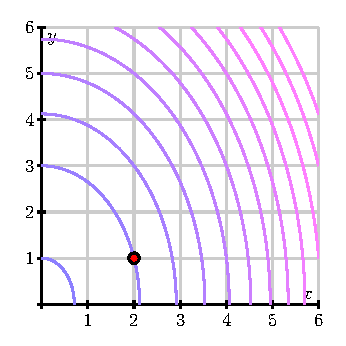
\includegraphics{figures/fig_10_6_preview_1.eps}
    \end{center}
    \caption{A contour plot of $f(x,y) = 30-x^2-\frac12 y^2$.}
    \label{F:10.6.preview.1}
  \end{figure}
  \ba
  	\item Suppose that a person is walking due east, and thus parallel to the $x$-axis.  At what instantaneous rate is the temperature changing at the moment she passes the point $(2,1)$?  What are the units on this rate of change?
	\item Next, determine the instantaneous rate of change of temperature at the point $(2,1)$ if the person is instead walking due north.  Again, include units on your result.
	\item Now, rather than walking due east or due north, let's suppose that the person is walking with velocity given by the vector $\vv = \langle 3, 4 \rangle$, where time is measured in seconds.  Note that the person's speed is thus $| \vv | = 5$ feet per second.
	
	Find parametric equations for the person's path; that is, parameterize the line through $(2,1)$ using the direction vector $\vv = \langle 3, 4 \rangle$.  Let $x(t)$ denote the $x$-coordinate of the line, and $y(t)$ its $y$-coordinate.
	
	\item With the parameterization in (c), we can now view the temperature $f$ as not only a function of $x$ and $y$, but also of time, $t$.  Hence, use the chain rule to determine the value of $\frac{df}{dt}\bigm|_{t=0}$.  What are the units on your answer?  What is the practical meaning of this result?
  \ea
  


\end{pa}

\begin{activitySolution} 
  \ba
  	\item The instantaneous rate of change in the temperature when a person is walking due east at the moment she passes the point $(2,1)$ is given by $f_x(2,1)$. Since $f_x(x,y) = -2x$, we have $f_x(2,1) = -4 \ \frac{^{\circ}C}{\text{foot}}$. 
  	
	\item The instantaneous rate of change in the temperature when a person is walking due north at the moment she passes the point $(2,1)$ is given by $f_y(2,1)$. Since $f_y(x,y) = -24 y$, we have $f_y(2,1) = -24 \ \frac{^{\circ}C}{\text{foot}}$. 
	
	\item Parametric equations for the line through $(2,1)$ in the direction of $\vv = \langle 3, 4 \rangle$ are
\[x(t) = 2 + 3t \ \text{ and } \ y(t)=1+4t.\]
	
	\item With the parameterization in (c), we have 
\[\frac{df}{dt} = \frac{\partial f}{\partial x} \frac{dx}{dt} + \frac{\partial f}{\partial y} \frac{dy}{dt} = (-2x)(3) - (24y)(4).\]
So
\[\frac{df}{dt}\biggm|_{t=0} = (-2)(2)(3) - (24)(1)(4) = -108 \ \frac{^{\circ}C}{\text{second}}.\]
So the temperature is decreasing by 108 degrees Celsius for every second she moves in the direction of $\vv$ from the point $(2,1)$. 
  \ea
\end{activitySolution}

 \afterpa 

\subsection*{Directional Derivatives}

Given a function $z = f(x,y)$, the partial derivative $f_x(x_0,y_0)$ measures the instantaneous rate of change of $f$ as only the $x$ variable changes; likewise, $f_y(x_0,y_0)$ measures the rate of change of $f$ at $(x_0,y_0)$ as only $y$ changes.  Note particularly that $f_x(x_0,y_0)$ is measured in ``units of $f$ per unit of change in $x$,'' and that the units on $f_y(x_0,y_0)$ are similar.  

In Preview Activity \ref{PA:10.6}, we saw how we could measure the rate of change of $f$ in a situation where both $x$ and $y$ were changing; in that activity, however, we found that this rate of change was measured in ``units of $f$ per unit of \emph{time}.'' In a given unit of time, we may move more than one unit of distance. In fact, in Preview Activity \ref{PA:10.6}, in each unit increase in time we move a distance of $| \vv | = 5$ feet. To generalize the notion of partial derivatives to any direction of our choice, we instead want to have a rate of change whose units are ``units of $f$ per unit of distance in the given direction.'' 

In this light, in order to formally define the derivative in a particular direction of motion, we want to represent the change in $f$ for a given \emph{unit} change in the direction of motion. We can represent this unit change in direction with a unit vector, say $\vu = \langle u_1, u_2 \rangle$.  If we move a distance $h$ in the direction of $\vu$ from a fixed point $(x_0,y_0)$, we then arrive at the new point $(x_0+u_1h, y_0+u_2h)$.  It now follows that the slope of the secant line to the curve on the surface through $(x_0,y_0)$ in the direction of $\vu$ through the points $(x_0,y_0)$ and $(x_0+u_1h, y_0+u_2h)$ is
\begin{equation}
m_{\mbox{sec}} = \frac{f(x_0+u_1h, y_0+u_2h) - f(x_0,y_0)}{h}. \label{eq:10.6.diff_quot}
\end{equation}

To get the instantaneous rate of change of $f$ in the direction $\vu = \langle u_1, u_2 \rangle$, we must take the limit of the quantity in Equation~\eqref{eq:10.6.diff_quot} as $h \to 0$.  Doing so results in the formal definition of the directional derivative.

\vspace*{5pt}
\nin \framebox{\hspace*{3 pt}
\parbox{6.25 in}{\begin{definition} Let $f = f(x,y)$ be given.  The \textbf{derivative of $f$ at the point $(x,y)$ in the direction of the unit vector $\vu = \langle u_1, u_2 \rangle$}\index{directional derivative} is denoted $D_{\vu}f(x,y)$ and is given by
\begin{equation} \label{E:DirDerDef}
D_{\vu}f(x,y) = \lim_{h \to 0} \frac{f(x+u_1h, y+u_2h) - f(x,y)}{h}
\end{equation}
for those values of $x$ and $y$ for which the limit exists. \end{definition}
} \hspace*{3 pt}}
\vspace*{5pt}

The quantity $D_{\vu} f(x,y)$ is called a \emph{directional derivative}. When we evaluate the directional derivative $D_{\vu} f(x,y)$ at a point $(x_0, y_0)$, the result $D_{\vu} f(x_0,y_0)$ tells us the instantaneous rate at which $f$ changes at $(x_0, y_0)$ per unit increase in the direction of the vector $\vu$. In addition, the quantity $D_{\vu} f(x_0,y_0)$  tells us the slope of the line tangent to the surface in the direction of $\vu$ at the point $(x_0,y_0,f(x_0,y_0))$.

\subsection*{Computing the Directional Derivative}

In a similar way to how we developed shortcut rules for standard derivatives in single variable calculus, and for partial derivatives in multivariable calculus, we can also find a way to evaluate directional derivatives without resorting to the limit definition found in Equation~\eqref{E:DirDerDef}.  We do so using a very similar approach to our work in Preview Activity~\ref{PA:10.6}.

Suppose we consider the situation where we are interested in the instantaneous rate of change of $f$ at a point $(x_0,y_0)$ in the direction $\vu = \langle u_1, u_2 \rangle$, where $\vu$ is a unit vector.   The variables $x$ and $y$ are therefore changing according to the parameterization
\[x = a + u_1t \ \ \ \ \ \text{ and } \ \ \ \ \  y = b + u_2t.\]
Observe that $\frac{dx}{dt} = u_1$ and $\frac{dy}{dt} = u_2$ for all values of $t$.  Since $\vu$ is a unit vector, it follows that a point moving along this line moves one unit of distance per one unit of time; that is, each single unit of time corresponds to movement of a single unit of distance in that direction.  This observation allows us to use the Chain Rule to calculate the directional derivative, which measures the instantaneous rate of change of $f$ with respect to change in the direction $\vu$.

In particular, by the Chain Rule, it follows that 
\[D_{\vu}f(x_0,y_0) = f_x(x_0,y_0)\frac{dx}{dt}\biggm|_{(x_0,y_0)} + f_y(x_0,y_0)\frac{dy}{dt}\biggm|_{(x_0,y_0)} = f_x(x_0,y_0)u_1 + f_y(x_0,y_0)u_2.\]
This now allows us to compute the directional derivative at an arbitrary point according to the following formula.

\vspace*{5pt}
\nin \framebox{\hspace*{3 pt}
\parbox{6.25 in}{Given a differentiable function $f = f(x,y)$ and a unit vector $\vu = \langle u_1, u_2 \rangle$, we may compute $D_{\vu}f(x,y)$  by
\begin{equation}
D_{\vu}f(x,y) = f_x(x,y)u_1 + f_y(x,y)u_2.\label{eq:10.6.DD}
\end{equation}
} \hspace*{3 pt}}
\vspace*{5pt}

\noindent \textbf{Note well:} To use Equation (\ref{eq:10.6.DD}), we must have a \emph{unit} vector $\vu = \langle u_1, u_2 \rangle$ in the direction of motion.  In the event that we have a direction prescribed by a non-unit vector, we must first scale the vector to have length 1.

\begin{activity} \label{A:10.6.2} Let $f(x,y) = 3xy-x^2y^3$.
	\ba
	
	\item Determine $f_x(x,y)$ and $f_y(x,y)$.
		
	\item Use Equation~\eqref{eq:10.6.DD} to determine $D_{\vi} f(x,y)$ and $D_{\vj} f(x,y)$. What familiar function is $D_{\vi} f(x,y)$? What familiar function is $D_{\vj} f(x,y)$?
	
	\item Use Equation~\eqref{eq:10.6.DD} to find the derivative of $f$ in the direction of the vector $\vv = \langle 2, 3 \rangle$ at the point $(1,-1)$.  Remember that a unit direction vector is needed.
	
%	\item Can you find a unit vector $\vw$ such that $D_{\vw} (1,-1) = 0$?
	
	
	\ea


\end{activity}
\begin{smallhint}

\end{smallhint}
\begin{bighint}

\end{bighint}
\begin{activitySolution}
\ba 
\item We have 
\[\frac{\partial f}{\partial x} = 3y-2xy^3 \ \ \text{ and } \ \ \frac{\partial f}{\partial y} = 3x - 3x^2y^2.\]

\item Since $\vi = \langle 1, 0 \rangle$, we have 
\[D_{\vi}f(x,y) = f_x(x,y)(1) + f_y(x,y)(0) = f_x(x,y).\]
So the derivative of $f$ in the direction of the vector $\vi$ is just the partial derivative of $f$ with respect to $x$.

Similarly,
\[D_{\vj}f(x,y) = f_x(x,y)(0) + f_y(x,y)(1) = f_y(x,y).\]
So the derivative of $f$ in the direction of the vector $\vj$ is just the partial derivative of $f$ with respect to $y$.

\item At the point $(1,-1)$ we have 
\[f_x(1,-1) = -1 \ \ \text{ and } \ \ f_y(1,-1) = 0.\]
So the derivative of $f$ in the direction of the unit vector $\frac{1}{|\vv|} \vv = \frac{1}{\sqrt{13}}\langle 2, 3 \rangle$ at the point $(1,-1)$ is
\[D_{\vv}f(1,-1) = f_x(1,-1) \left(\frac{2}{\sqrt{13}}\right) + f_y(1,-1) \left(\frac{3}{\sqrt{13}}\right) = -\frac{2}{\sqrt{13}}.\]

\ea
 
\end{activitySolution}
\aftera

\subsection*{The Gradient}

Via the Chain Rule, we have seen that for a given function $f = f(x,y)$, its instantaneous rate of change in the direction of a unit vector $\vu = \langle u_1, u_2 \rangle$ is given by 
\begin{equation} \label{E:DDrevisited}
D_{\vu}f(x_0,y_0) = f_x(x_0,y_0)u_1 + f_y(x_0,y_0)u_2.
\end{equation}
Recalling that the dot product of two vectors $\vv = \langle v_1, v_2 \rangle$ and $\vu = \langle u_1, u_2 \rangle$ is computed by 
$$\vv \cdot \vu = v_1 u_1 + v_2 u_2,$$
we see that we may recast Equation~\eqref{E:DDrevisited} in a way
  that has geometric meaning.  In particular, we see that $D_{\vu}f(x_0,y_0)$ is the dot product of the vector $\left\langle f_x(x_0,y_0), f_y(x_0,y_0) \right\rangle$ and the vector $\vu$.
  
 We call this
  vector formed by the partial derivatives of $f$ the {\em gradient} of $f$ and denote it
  $$
  \nabla f(x_0,y_0) = \left\langle f_x(x_0,y_0), f_y(x_0,y_0) \right\rangle.
  $$
We read $\nabla f$ as ``the gradient of $f$,'' ``grad $f$" or ``del $f$".\footnote{The symbol
  $\nabla$ is called \emph{nabla}, which comes from a Greek word for a
  certain type of harp that has a similar shape.}  
Notice that $\nabla f$ varies from point to point.  In the following activity, we investigate some of what the gradient tells us about the behavior of a function $f$.

\newpage

\begin{activity} \label{A:10.6.10} 
  Let's consider the function $f$ defined  by $f(x,y) = x^2 - y^2$.  Some contours for this function are shown in Figure
  \ref{F:10.6.activity.1}. 

  \begin{figure}[ht]
    \begin{center}
      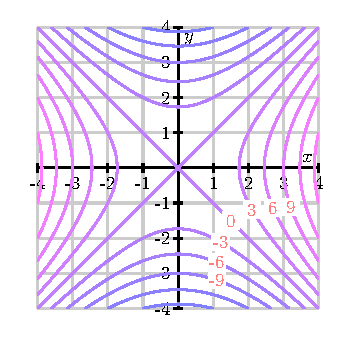
\includegraphics{figures/fig_10_6_contours_1.eps}
    \end{center}	
    \caption{Contours of $f(x,y) = x^2 - y^2$. }
    \label{F:10.6.activity.1}
  \end{figure}
  \ba
  \item Find the gradient $\nabla f (x,y)$.
  \item For each of the following points $(x_0,y_0)$, evaluate the gradient $\nabla f(x_0,y_0)$ and sketch the gradient vector with its tail at
    $(x_0,y_0)$.  Some of the vectors are too long
    to fit onto the plot, but we'd like to draw them to scale;  to do so, scale each vector by a factor of 1/4.
    \begin{itemize}
      \item $(x_0,y_0) = (2,0)$
      \item $(x_0,y_0) = (0,2)$
      \item $(x_0,y_0) = (2,2)$
      \item $(x_0,y_0) = (2,1)$
      \item $(x_0,y_0) = (-3,2)$
      \item $(x_0,y_0) = (-2,-4)$
      \item $(x_0,y_0) = (0,0)$
    \end{itemize}
  \item What do you notice about the relationship between the gradient at
    $(x_0,y_0)$ and the contour line passing through that point?
  \item Does $f$ increase or decrease in the direction of $\nabla
    f(x_0,y_0)$?  Provide a justification for your response.

    \ea

\end{activity}

\begin{activitySolution}
\ba 
\item By definition, 
\[\nabla f (x,y) = \langle f_x(x,y), f_y(x,y) \rangle = \langle 2x, -2y \rangle.\]

\item We apply the formula for the gradient to see that 
\begin{align*}
\nabla f(2,0) &= \langle 4,0 \rangle \\
\nabla f(0,2) &= \langle 0,-4 \rangle \\
\nabla f(2,2) &= \langle 4,-4 \rangle \\
\nabla f(2,1) &= \langle 4,-2 \rangle \\
\nabla f(-3,2) &= \langle -3,-4 \rangle \\
\nabla f(-2,-4) &= \langle -4,8 \rangle \\
\nabla f (0,0) &= \langle 0,0 \rangle.
\end{align*}
A picture of the scaled gradients are shown here. 
   \begin{center}
      \resizebox{!}{2.4in}{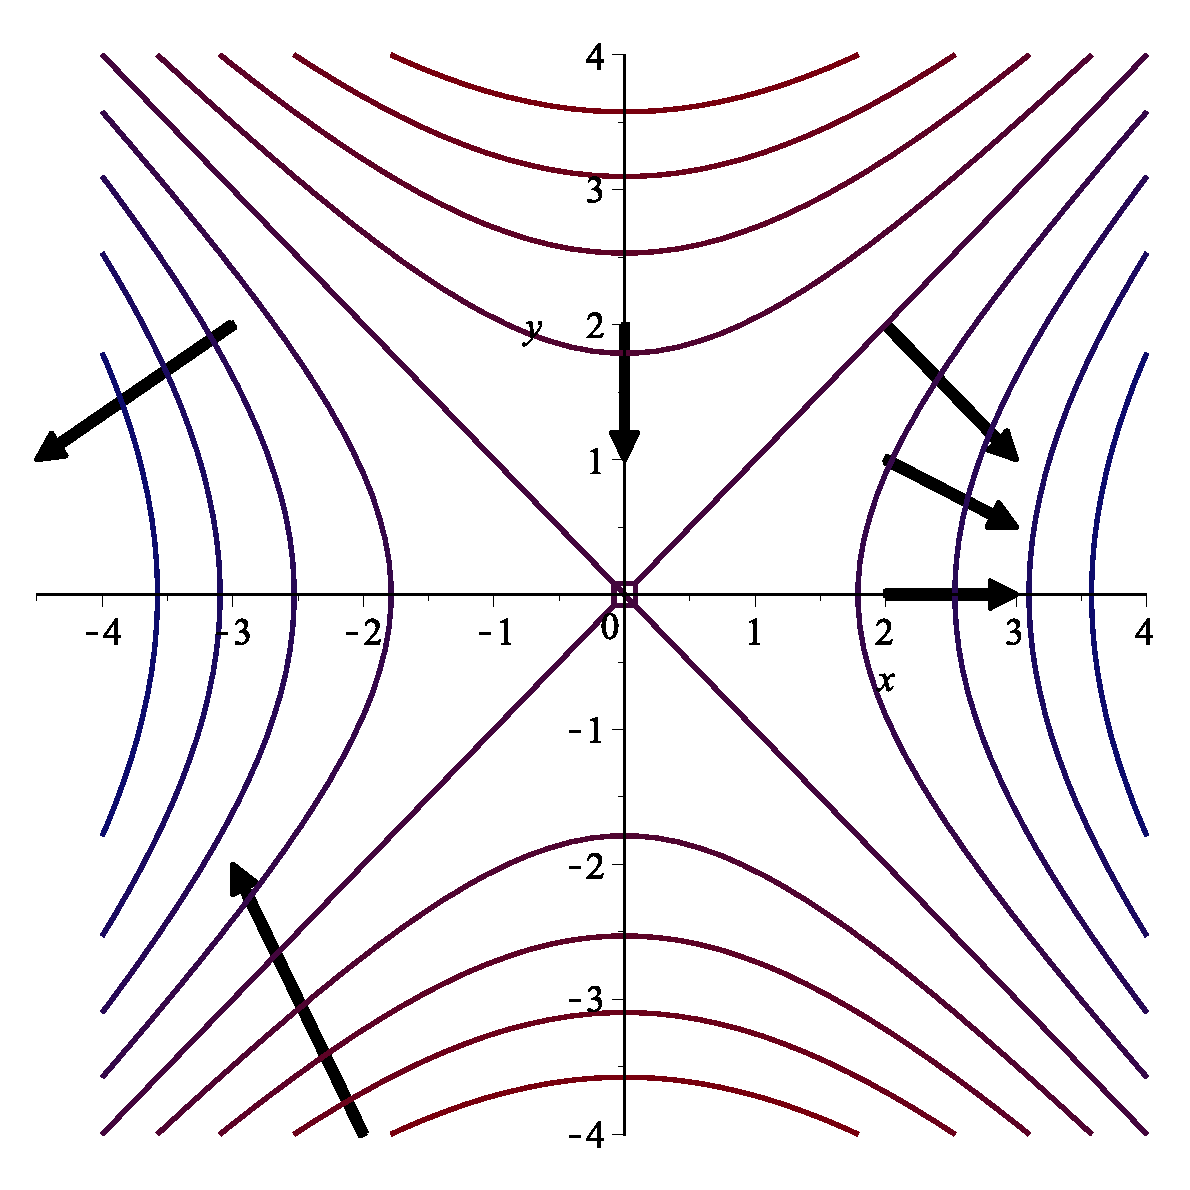
\includegraphics{figures/fig_10_6_Act_10_contours.eps}}
    \end{center}
\item It appears that each gradient is orthogonal to the contour containing its tail.
\item In the first quadrant, as $x$ increases so does $f(x,y)$. So these gradients all point in a direction of increase of $f$. In the second quadrant, as $x$ decreases $f(x,y)$ increases. So these gradients all point in a direction of increase of $f$. In the third quadrant, as $y$ increases so does $f(x,y)$. So these gradients all point in a direction of increase of $f$. Finally, at the point $(0,2)$, $f$ increases as $y$ decreases. So every gradient points in a direction of increase of $f$.
\ea
 
\end{activitySolution}
\aftera


As a vector, $\nabla f(x_0,y_0)$ defines a direction and a length.  As we will soon see, both
of these convey important information about the behavior of $f$ near
$(x_0,y_0)$.  

\subsection*{The Direction of the Gradient}

Remember that the dot product also conveys information about the angle
between the two vectors.  If $\theta$ is the angle between $\nabla
f(x_0,y_0)$ and $\vu$ (where $\vu$ is a unit vector), %as shown in Figure \ref{F:10.6.gradient.1},
then we also have that
$$
D_{\vu}f(x_0,y_0) = \nabla f(x_0,y_0)\cdot\vu = |\nabla f(x_0,y_0)||\vu|
\cos\theta.
$$

%  \begin{figure}[ht]
%    \begin{center}
 %     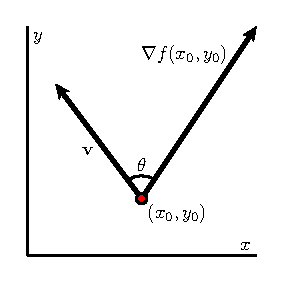
\includegraphics{figures/fig_10_6_gradient_angle.eps}
 %   \end{center}	
 %   \caption{The angle between $\nabla f(x_0,y_0)$ and $\vv$. }
 %   \label{F:10.6.gradient.1}
%  \end{figure}

In particular, when $\theta$ is a right angle, as shown on the left of
Figure \ref{F:10.6.gradient.sign}, then $D_{\vu}f(x_0,y_0) = 0$, because $\cos(\theta) = 0$.  Since the value of the directional derivative is 0, this means that $f$ is unchanging in this direction, and hence $\vu$ must be tangent to the contour of $f$ that passes through $(x_0,y_0)$.  In other words, $\nabla f(x_0,y_0)$ is orthogonal to the
contour through $(x_0,y_0)$.  This shows that the gradient vector at a given point is always perpendicular to the contour passing through the point, confirming that what we saw in part (c) of Activity~\ref{A:10.6.10} holds in general.

  \begin{figure}[ht]
    \begin{center}
      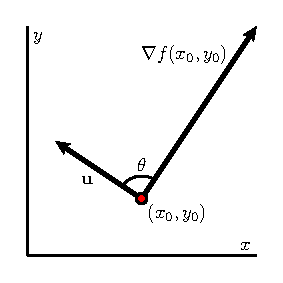
\includegraphics{figures/fig_10_6_gradient_angle_1.eps}
      \hspace*{20pt}
      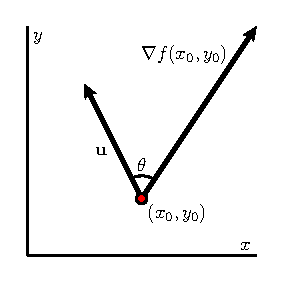
\includegraphics{figures/fig_10_6_gradient_angle_2.eps}
      \hspace*{20pt}
      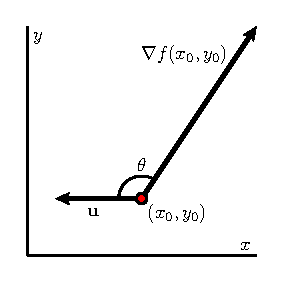
\includegraphics{figures/fig_10_6_gradient_angle_3.eps}
    \end{center}	
    \caption{The sign of $D_{\vu} f(x_0,y_0)$ is determined by $\theta$.}
    \label{F:10.6.gradient.sign}
  \end{figure}

Moreover, when $\theta$ is an acute angle, it follows that $\cos\theta > 0$ so since $$
D_{\vu}f(x_0,y_0) = |\nabla f(x_0,y_0)||\vu|
\cos\theta,
$$
and therefore $D_{\vu}f(x_0,y_0) > 0$, as shown in the middle image in Figure
\ref{F:10.6.gradient.sign}.  This means that $f$ is increasing in any direction where
$\theta$ is acute.  In a similar way, when $\theta$ is an obtuse angle, then $\cos\theta < 0$ so $D_{\vu}f(x_0,y_0) < 0$, as seen on the right in Figure \ref{F:10.6.gradient.sign}.  This
means that $f$ is decreasing in any direction for which $\theta$ is obtuse.

Finally, as we can see in the following activity, we may also use the gradient to determine the directions in which the function is increasing and decreasing most rapidly.

\begin{activity} \label{A:10.6.3} In this activity we investigate how the gradient is related to the directions of greatest increase and decrease of a function.  Let $f$ be a differentiable function and $\vu$ a unit vector.
\ba
    \item Let $\theta$ be the angle between $\nabla f(x_0,y_0)$ and $\vu$.  Explain why
\begin{equation}
D_{\vu} f(x_0,y_0) = |\langle f_x(x_0,y_0), f_y(x_0,y_0) \rangle | \cos(\theta). \label{eq:10.6.DD_grad2}
\end{equation}

    \item At the point $(x_0,y_0)$, the only quantity in Equation~(\ref{eq:10.6.DD_grad2}) that can change is $\theta$ (which determines the direction $\vu$ of travel). Explain why $\theta = 0$ makes the quantity 
\[|\langle f_x(x_0,y_0), f_y(x_0,y_0) \rangle| \cos(\theta)\]
as large as possible.


    \item When $\theta = 0$, in what direction does the unit vector $\vu$ point relative to $\nabla f(x_0,y_0)$? Why? What does this tell us about the direction of greatest increase of $f$ at the point $(x_0,y_0)$?
    
    \item In what direction, relative to $\nabla f(x_0,y_0)$, does $f$ decrease most rapidly at the point $(x_0,y_0)$?
    
    \item State the unit vectors $\vu$ and $\vv$ (in terms of $\nabla f(x_0,y_0)$) that provide the directions of greatest increase and decrease for the function $f$ at the point $(x_0,y_0)$.  What important assumption must we make regarding $\nabla f(x_0,y_0)$ in order for these vectors to exist?


    \ea



\end{activity}
\begin{smallhint}

\end{smallhint}
\begin{bighint}

\end{bighint}
\begin{activitySolution}
\ba 
\item Using the dot product we can see that
\[D_{\vu} f(x_0,y_0) = \langle f_x(x_0,y_0), f_y(x_0,y_0) \rangle \cdot \vu = |\langle f_x(x_0,y_0), f_y(x_0,y_0) \rangle| \cos(\theta),\]
where $\theta$ is the angle between $\langle f_x(x_0,y_0), f_y(x_0,y_0) \rangle$ and $\vu$.

\item The maximum value of $D_{\vu} f(x_0,y_0)$ will occur when $\cos(\theta)$ is as large as possible. This happens when $\cos(\theta) = 1$ or $\theta = 0$.

\item When $\theta = 0$, the angle between the vector $\vu$ and the vector $\langle f_x(x_0,y_0), f_y(x_0,y_0) \rangle$ is 0, so the vector $\vu$ must have the same direction as $\langle f_x(x_0,y_0), f_y(x_0,y_0) \rangle$. In other words, the direction of greatest increase of $f$ at the point $(x_0,y_0)$ is the direction of the vector $\langle f_x(x_0,y_0), f_y(x_0,y_0) \rangle$.

\item If $f$ increases most rapidly in the direction of $\langle f_x(x_0,y_0), f_y(x_0,y_0) \rangle$ at the point $(x_0,y_0)$, then $f$ must decrease most rapidly in the opposite direction, or in the direction of $-langle f_x(x_0,y_0), f_y(x_0,y_0) \rangle$.

\item The unit vector that provides the direction of greatest increase in $f$ at the point $(x_0,y_0)$ is $\vu=\frac{1}{|\nabla f(x_0,y_0)|} \nabla f(x_0,y_0)$ and the unit vector that provides the direction of greatest decrease in $f$ at the point $(x_0,y_0)$ is $\vv = -\vu$. For either vector to exist, it must be the case that $\nabla f(x_0,y_0) \neq \langle 0,0 \rangle$. 
\ea

\end{activitySolution}
\aftera


%\begin{activity} \label{A:10.6.12} 
  Figure \ref{F:10.6.gradient.field} shows a plot of the gradient
  $\nabla f$ at several points for some function $f(x,y)$.

  \begin{figure}[ht]
    \begin{center}
      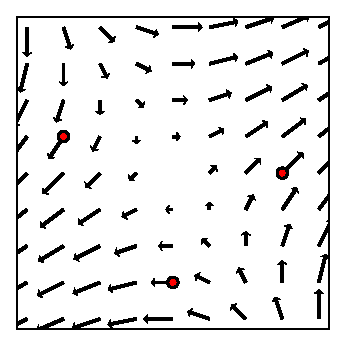
\includegraphics{figures/fig_10_6_gradient_field.eps}
    \end{center}	
    \caption{The gradient $\nabla f$.}
    \label{F:10.6.gradient.field}
  \end{figure}

  \ba
\item Consider each of the three indicated points, and draw, as best
  as you can, the contour line through that point.

\item Beginning at each point, draw a curve on which $f$ is continually
  decreasing. 

  \ea

\end{activity}
\aftera


\subsection*{The Length of the Gradient}

Having established in Activity~\ref{A:10.6.3} that the direction in which a function increases most rapidly at a point $(x_0,y_0)$ is the unit vector $\vu$ in the direction of the gradient, (that is, $\vu = \frac{1}{|\nabla f(x_0,y_0)|} \nabla f(x_0,y_0)$, provided that $\nabla f(x_0,y_0) \ne \vzero$), it is also natural to ask, ``in the direction of greatest increase for $f$ at $(x_0,y_0)$, what is the \emph{value} of the rate of increase?''  In this situation, we are asking for the value of $D_{\vu} f(x_0,y_0)$ where $\vu = \frac{1}{|\nabla f(x_0,y_0)|} \nabla f(x_0,y_0)$.

Using the now familiar way to compute the directional derivative, we see that
$$D_{\vu} f(x_0,y_0) = \nabla f(x_0,y_0) \cdot \left(\frac{1}{|\nabla f(x_0,y_0)|} \nabla f(x_0,y_0) \right).$$
Next, we recall two important facts about the dot product:  (i) $\vw\cdot (c \vv) = c (\vw \cdot \vv)$ for any scalar $c$, and (ii) $\vw \cdot \vw = |\vw|^2$.  Applying these properties to the most recent equation involving the directional derivative, we find that 
$$D_{\vu} f(x_0,y_0) = \frac{1}{|\nabla f(x_0,y_0)|}  (\nabla f(x_0,y_0) \cdot \nabla f(x_0,y_0)) = \frac{1}{|\nabla f(x_0,y_0)|} |\nabla f(x_0,y_0)|^2. $$
Finally, since $\nabla f(x_0,y_0)$ is a nonzero vector, its length $|\nabla f(x_0,y_0)|$ is a nonzero scalar, and thus we can simplify the preceding equation to establish that
$$D_{\vu} f(x_0,y_0) = |\nabla f(x_0,y_0)|.$$
We summarize our most recent work by stating two important facts about the gradient.

\vspace*{5pt}
\nin \framebox{\hspace*{3 pt}
\parbox{6.25 in}{
Let $f$ be a differentiable function and $(x_0,y_0)$ a point for which $\nabla f(x_0,y_0) \ne \vzero$.  Then $\nabla f(x_0,y_0)$ points in the direction of greatest increase of $f$ at $(x_0,y_0)$, and the instantaneous rate of change of $f$ in that direction is the length of the gradient vector.  That is, if $\vu = \frac{1}{|\nabla f(x_0,y_0)|} \nabla f(x_0,y_0)$, then $\vu$ is a unit vector in the direction of greatest increase of $f$ at $(x_0,y_0)$, and $D_{\vu} f(x_0,y_0) = |\nabla f(x_0,y_0)|$.
} \hspace*{3 pt}}
\vspace*{5pt}

%\newpage

\begin{activity} \label{A:10.6.11} 
  Consider the function $f$ defined by $f(x,y) = 2x^2 - xy + 2y$.  
  \ba
\item Find the gradient $\nabla f(1,2)$ and sketch it on Figure
  \ref{F:10.6.activity.empty}. 

  \begin{figure}[ht]
    \begin{center}
      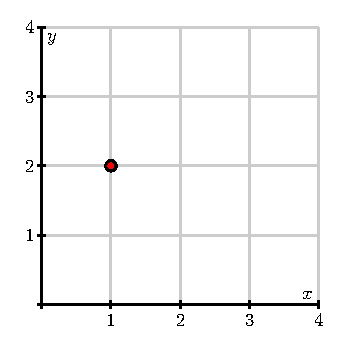
\includegraphics{figures/fig_10_6_activity_empty.eps}
    \end{center}	
    \caption{A plot for the gradient $\nabla f(1,2)$.}
    \label{F:10.6.activity.empty}
  \end{figure}

\item Sketch the unit vector $\vz = \left\langle-\frac1{\sqrt{2}},
    -\frac1{\sqrt{2}}\right\rangle$ on Figure
  \ref{F:10.6.activity.empty} with its tail at $(1,2)$.
  Now find the directional derivative $D_{\vz}f(1,2)$.  

\item What is the slope of the graph of $f$ in the direction $\vz$?  
  What does the sign of the directional derivative tell you?  

\item Consider the vector $\vv = \langle 2,-1\rangle$ and sketch $\vv$
  on Figure \ref{F:10.6.activity.empty} with its tail at $(1,2)$.
  Find a unit vector $\vw$ pointing in the same direction of $\vv$.
  Without computing $D_{\vw}f(1,2)$, what do you know about the sign
  of this directional derivative?  Now verify your observation by
  computing $D_{\vw}f(1,2)$.

\item 
%If $\theta$ is the angle between $\nabla f(1,2)$ and $\vu$, then
%  $$
%  D_{\vu}f(1,2) = \nabla f(1,2)\cdot \vu = |\nabla
 % f(1,2)||\vu|\cos\theta = |\nabla
%  f(1,2)|\cos\theta,
 % $$
 % since $\vu$ is a unit vector.  
 In which direction (that is, for what unit vector $\vu$) is $D_{\vu}f(1,2)$
  the greatest?  What is the slope of the graph in this direction?

\item Corresponding, in which direction is $D_{\vu}f(1,2)$ least?  What is the slope of the graph in this direction?

\item Sketch two unit vectors $\vu$ for which $D_{\vu}f(1,2) = 0$ and
  then find component representations of these vectors.

\item Suppose you are standing at the point $(3,3)$.  In which
  direction should you move to cause $f$ to increase as rapidly as
  possible?  At what rate does $f$ increase in this direction?

  \ea

\end{activity}

\begin{activitySolution}
\ba 
\item The gradient of $f$ at $(1,2)$ is
\[\nabla f(1,2) = \langle f_x(1,2), f_y(1,2) \rangle = \langle 2,1\rangle.\]
A plot of  $\nabla f(1,2)$ is shown below.

\item A plot of $\vz$ is shown below. The directional derivative $D_{\vz}f(1,2)$ is 
\[D_{\vz}f(1,2) = f_x(1,2)\left(-\frac{1}{\sqrt{2}}\right) + f_y(1,2)\left(-\frac{1}{\sqrt{2}}\right) = -\frac{3}{\sqrt{2}}.\]

\item The directional derivative $D_{\vz}f(1,2)$ tells us the slope of $f$ in the direction of $\vz$ at the point $(1,2)$, so this slope is $-\frac{3}{\sqrt{2}}$. The fact that $D_{\vz}f(1,2)$ is negative tells us that the graph of $f$ is decreasing in the direction of $\vz$ from the point $(1,2)$. 

\item The angle between the vector $\vv$ or the vector $\vw = \frac{1}{|\vv|} \vv = \frac{1}{\sqrt{5}}\langle 2, -1 \rangle$ (shown below) and $\nabla f(1,2)$ is acute, so we expect $f$ to be increasing in this direction. Note that 
\[D_{\vw}f(1,2) = \frac{1}{\sqrt{5}}(f_x(1,2)(2) + f_y(1,2)(-1)) = \frac{3}{5}\sqrt{5}.\] 

   \begin{center}
      \resizebox{!}{2.4in}{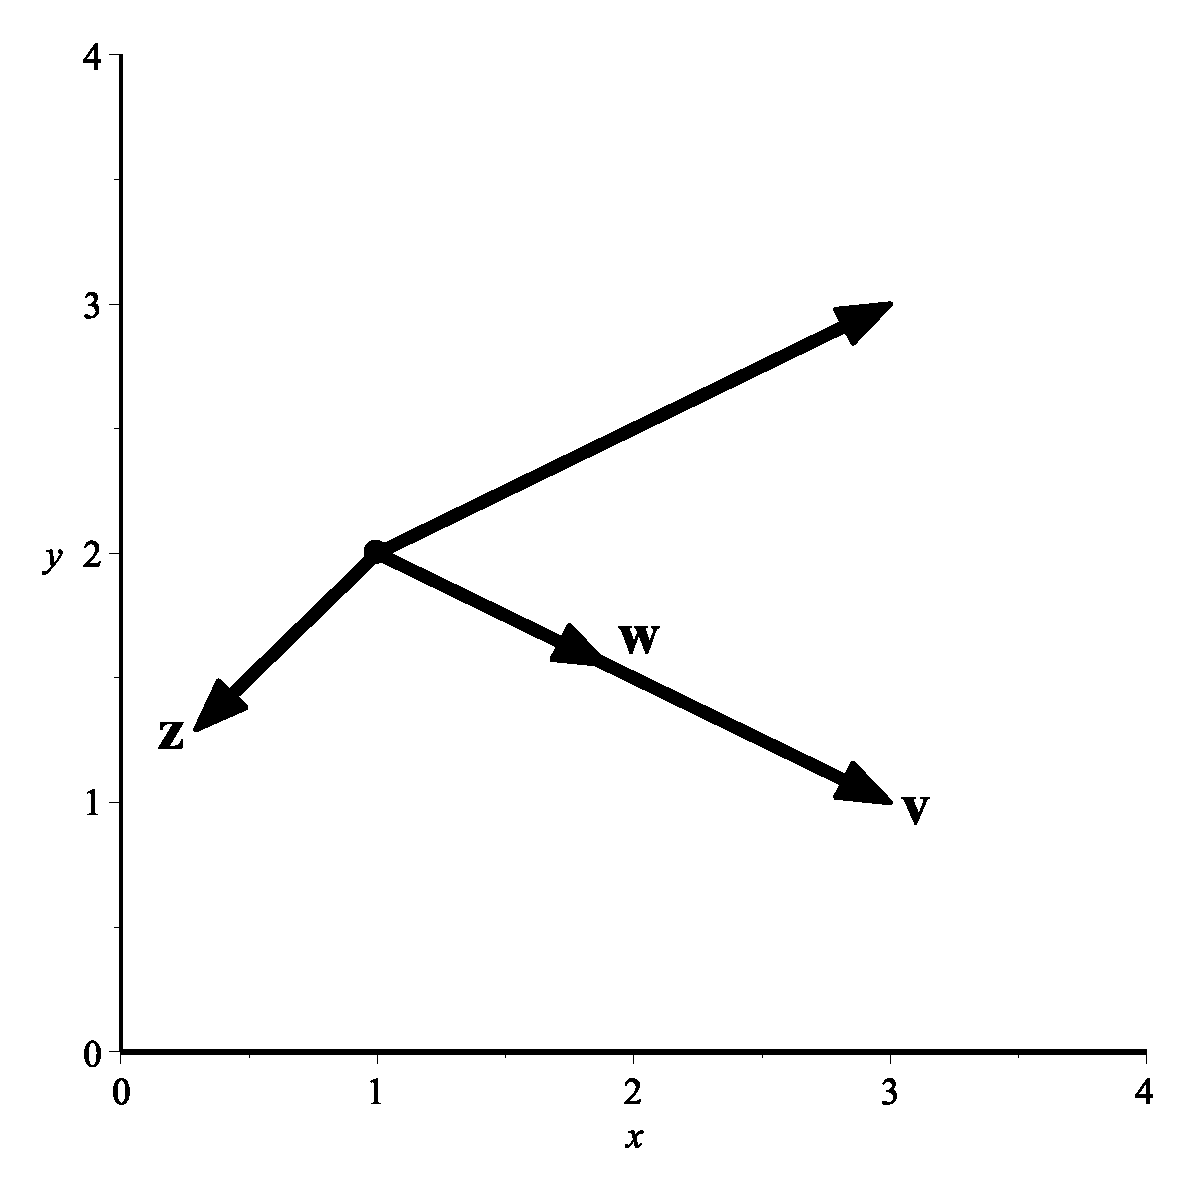
\includegraphics{figures/fig_10_6_Act_11_gradient.eps}}
    \end{center}
    
\item We know that $f$ increases most rapidly in the direction of the gradient. So $D_{\vu}f(1,2)$ is greatest when \[\vu = \frac{1}{|\nabla f(1,2)|} \nabla f(1,2) =  \frac{1}{\sqrt{5}}\langle 2,1 \rangle.\]
The slope of the graph of $f$ in the direction of $\nabla f(1,2)$ at the point $(1,2)$ is
\[D_{\vu}f(1,2) = \frac{1}{|\nabla f(1,2)|}(f_x(1,2)(f_x(1,2)) + f_y(1,2)(f_y(1,2))) = |\nabla f(1,2)| = \sqrt{5}.\]

\item the function $f$ decreases most rapidly in the direction opposite of the gradient. So $D_{\vu}f(1,2)$ is least when 
\[\vu = -\frac{1}{|\nabla f(1,2)|} \nabla f(1,2) =  -\frac{1}{\sqrt{5}}\langle 2,1 \rangle.\]
The slope of the graph of $f$ in the direction of $-\nabla f(1,2)$ at the point $(1,2)$ is
\[D_{\vu}f(1,2) = - |\nabla f(1,2)| = -\sqrt{5}.\] 

\item Recall that $D_{\vu}f(1,2) = \nabla f(1,2) \cdot \vu$, so $D_{\vu}f(1,2) = 0$ when $\vu$ is perpendicular to $\nabla f(1,2)$. By inspection, two such vectors are $\frac{1}{\sqrt{5}}\langle 1, -2 \rangle$ and $\frac{1}{\sqrt{5}}\langle -1,2 \rangle$.  

\item The direction in which $f$ increases most rapidly at the point $(3,3)$ is 
\[\vu=\frac{1}{|\nabla f(3,3)|}\nabla f(3,3) = \frac{1}{\sqrt{82}}\langle 9, -1 \rangle.\]
The rate of increase of $f$ in this direction is 
\[D_{\vu} f (3,3) = |\nabla f(3,3)| = \sqrt{82}.\]
\ea

\end{activitySolution}

\aftera


  
%\begin{activity} \label{A:10.6.14} 
  Suppose that the temperature in a region of space is described by
  $$
  T(x,y,z) = 100e^{-x^2-y^2-z^2}
  $$
  and that you are standing at the point $(1,2,-1)$.
  \ba
\item Find the rate of change of the temperature in the direction of
  $\vv=\langle 0, 1, 2\rangle$.  Remember that you should first find a
  {\em unit} vector in the direction of $\vv$.

\item In what direction would you move to cause the temperature to
  decrease as quickly as possible?

\item How fast does the temperature decrease in this direction?

\item Find a direction in which the temperature does
  not change.

  \ea

\end{activity}
\aftera


\subsection*{Applications}

The gradient finds many natural applications.  For example, situations often arise -- for instance, constructing a road through the mountains or planning the flow of water across a landscape -- where we are
interested in knowing the direction in which a function is increasing
or decreasing most rapidly. 

For example, consider a two-dimensional version of how a heat-seeking
missile might work.\footnote{This application is borrowed from United
  States Air Force Academy Department of Mathematical Sciences at
  \url{http://www.nku.edu/~longa/classes/mat320/mathematica/multcalc.htm}.}
Suppose that the temperature surrounding a fighter jet can be
modeled by the function $T$ defined by
\[T(x,y) = \frac{100}{1+(x-5)^2 + 4(y-2.5)^2},\] where $(x,y)$ is a
point in the plane of the fighter jet and $T(x,y)$ is measured in
degrees 
Celsius.  Some contours and gradients $\nabla T$ are shown on
the left in Figure \ref{F:10.6.missile}.

  \begin{figure}[ht]
    \begin{center}
      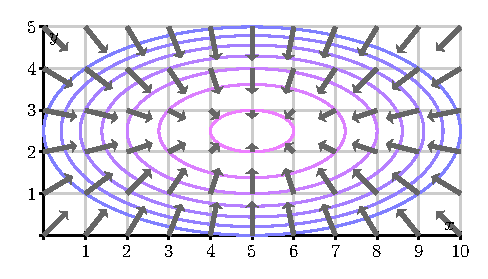
\includegraphics{figures/fig_10_6_missile_grad.eps}
      \hspace*{20pt}
      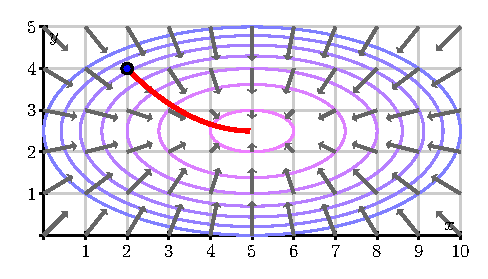
\includegraphics{figures/fig_10_6_missile_path.eps}
    \end{center}	
    \caption{Contours and gradient for $T(x,y)$ and the missile's path.}
    \label{F:10.6.missile}
  \end{figure}

A heat-seeking missile will always travel in the direction in which
the temperature increases most rapidly;  that is, it will always
travel in the direction of the gradient $\nabla T$.  If a missile is
fired from the point $(2,4)$, then its path will be that shown on the
right in Figure \ref{F:10.6.missile}.

In the final activity of this section, we consider several questions related to this context of a heat-seeking missile, and foreshadow some upcoming work in Section~\ref{S:10.7.Optimization}.

\begin{activity} \label{A:10.6.13} 
  \ba
\item The temperature $T(x,y)$ has its maximum value at the fighter
  jet's location.  State the fighter jet's location and explain
  how Figure \ref{F:10.6.missile} tells you this.
\item Determine $\nabla T$ at the fighter jet's location and give a
  justification for your response.
\item Suppose that a different function $f$ has a local maximum value at
  $(x_0,y_0)$.  Sketch the behavior of some possible contours near this point. 
  What is $\nabla f(x_0,y_0)$?
\item Suppose that a function $g$ has a local minimum value at
  $(x_0,y_0)$.  Sketch the behavior of some possible contours near this point.
  What is $\nabla g(x_0,y_0)$?
\item If a function $g$ has a local minimum at  $(x_0,y_0)$, what is the direction of greatest increase of $g$ at $(x_0,y_0)$?
  \ea

\end{activity}

\begin{activitySolution}
\ba 
\item The gradient points toward the direction of greatest in $T$, and the gradient vectors are all directed toward the point $(5,2.5)$. So the fighter jet's location is $(5,2.5)$. 

\item At the fighter jet's location, the temperature doesn't increase, so we should expect $\nabla T$ to be the zero vector there. Note that $T_x(x,y) = -\frac{200(x-5)}{[1+(x-5)^2+4(y-2.5)^2]^2}$ and $T_y(x,y) =  -\frac{800(y-2.5)}{[1+(x-5)^2+4(y-2.5)^2]^2}$, and so $\nabla T(5,2.5) = \langle 0, 0 \rangle$. 

\item Contours of $f$ might look like the contours of $T$ near the point $(x_0,y_0)$. At the relative maximum point we would have $\nabla f(x_0,y_0) = \langle 0,0\rangle$, provided $\nabla f(x_0,y_0)$ exists.

\item Contours of $g$ might look like the contours of $T$ near the point $(x_0,y_0)$ only with the gradients pointing outward instead of inward. At the relative maximum point we would have $\nabla g(x_0,y_0) = \langle 0,0\rangle$, provided $\nabla g(x_0,y_0)$ exists.

\item If $g$ has a local minimum at $(x_0,y_0)$ and $\nabla g(x_0,y_0) = \langle 0,0 \rangle$, then any direction will provide the greatest increase in $g$ at the point $(x_0,y_0)$.  
\ea

\end{activitySolution}

\aftera


\begin{summary}

\item The directional derivative of $f$ at the point $(x,y)$ in the direction of the unit vector $\vu = \langle u_1, u_2 \rangle$ is 
\begin{equation*}
D_{\vu}f(x,y) = \lim_{h \to 0} \frac{f(x+u_1h, y+u_2h) - f(x,y)}{h}
\end{equation*}
for those values of $x$ and $y$ for which the limit exists.  In addition, $D_{\vu}f(x,y)$ measures the slope of the graph of $f$ when we move in the direction
  $\vu$.   Alternatively, $D_{\vu} f(x_0,y_0)$ measures the instantaneous rate of change of $f$ in the direction $\vu$ at $(x_0,y_0)$.

\item The gradient of a function $f(x,y)$ at a point $(x_0,y_0)$ is
  the vector
  $$
  \nabla f(x_0,y_0) = \left\langle f_x(x_0,y_0),
    f_y(x_0,y_0)\right\rangle.
  $$

\item The directional derivative in the direction $\vu$ may be computed by
  $$D_{\vu}f(x_0,y_0) = \nabla f(x_0,y_0)\cdot \vu.
  $$
  

\item At any point where the gradient is nonzero,  gradient is orthogonal to the contour through
  that point and points in the direction in which $f$ increases most
  rapidly; moreover, the slope of $f$ in this direction equals the length of the
  gradient $|\nabla f(x_0,y_0)|$.  Similarly, the opposite of the gradient points in the direction of greatest decrease, and that rate of decrease is the opposite of the length of the gradient.
\end{summary}





\nin \hrulefill

\begin{exercises} 


\item Let $E(x,y) = \ds \frac{100}{1+(x-5)^2 + 4(y-2.5)^2}$ represent the elevation on a land mass at location $(x,y)$.  Suppose that $E$, $x$, and $y$ are all measured in meters.
    \ba
    \item Find $E_x(x,y)$ and $E_y(x,y)$.

    \item Let $\vu$ be a unit vector in the direction of $\langle -4,3 \rangle$.  Determine $D_{\vu} E(3,4)$.  What is the practical meaning of $D_{\vu} E(3,4)$ and what are its units?

    \item Find the direction of greatest increase in $E$ at the point $(3,4)$.

    \item Find the instantaneous rate of change of $E$ in the direction of greatest decrease at the point $(3,4)$.  Include units on your answer.
    
    \item At the point $(3,4)$, find a direction $\vw$ in which the instantaneous rate of change of $E$ is 0.

    \ea

\begin{exerciseSolution}
\ba 
\item For this function $E$ we have 
\[E_x(x,y) = -\frac{200(x-5)}{(1+(x-5)^2 + 4(y-2.5)^2)^2} \ \ \text{ and } \ \ E_y(x,y) = -\frac{800(y-2.5)}{(1+(x-5)^2 + 4(y-2.5)^2)^2}.\]

\item A unit vector in the direction of $\langle -4,3 \rangle$ is $\vu = \frac{1}{5} \langle -4, 3 \rangle$. Since
\[E_x(3,4) = \frac{100}{49} \ \ \text{ and } \ \ E_y(3,4) = -\frac{300}{49},\]
we have
\[D_{\vu} E(3,4) = \nabla E(3,4) \cdot \vu = \left\langle \frac{100}{49}, -\frac{300}{49} \right\rangle \cdot \frac{1}{5} \langle -4,3 \rangle = \frac{20}{49} (-4 - 9) = -\frac{260}{49} \approx -5.306 \ \frac{\text{meters}}{\text{meter}}.\]
For every one meter change in the direction of $\vu$ from the point $(3,4)$, the elevation decreases by $\frac{260}{49}$ meters. 
 
\item The direction of greatest increase of $E$ at the point $(3,4)$ is 
\[\nabla E (3,4) = \langle E_x(3,4), E_y(3,4) \rangle = \frac{100}{49} \langle 1, -3 \rangle \approx \langle 2.04, -6.12 \rangle.\]

\item The direction of greatest decrease of $E$ at $(3,4)$ is $-\nabla E(3,4)$. The instantaneous rate of change of $E$ in the direction of greatest decrease at the point $(3,4)$ is
\[-|\nabla E(3,4)| = -\frac{100}{49}\sqrt{1+9} = -\frac{100}{49}\sqrt{10} \approx -6.454 \ \frac{\text{meters}}{\text{meter}}.\]

\item We want a direction vector $\vw = \langle w_1, w_2 \rangle$ so that 
\[0 = D_{\vw} E(3,4) = \nabla E(3,4) \cdot \vw = \left\langle \frac{100}{49}, -\frac{300}{49} \right\rangle \cdot \langle w_1, w_2 \rangle = \frac{100}{49}(w_1-3w_2).\]
So the vector $\langle 3, 1 \rangle$ is a direction in which $E$ does not change at the point $(3,4)$.
\ea


\end{exerciseSolution}

\item Let $f(x,y) = x^2+3y^2$.
    \ba
    \item Find $\nabla f(x,y)$ and $\nabla f(1,2)$.

    \item Find the direction of greatest increase in $f$ at the point $(1,2)$. Explain. A graph of the surface defined by $f$ is shown in Figure \ref{F:10.6.Grad_ex}. Illustrate this direction on the surface.

    \item A contour diagram of $f$ is shown in Figure \ref{F:10.6.Grad_ex_contours}. Illustrate your calculation from (b) on this contour diagram.
\begin{figure}[ht]
\begin{center}
\begin{minipage}{2.5in}
\begin{center}
%\resizebox{!}{2.4in}{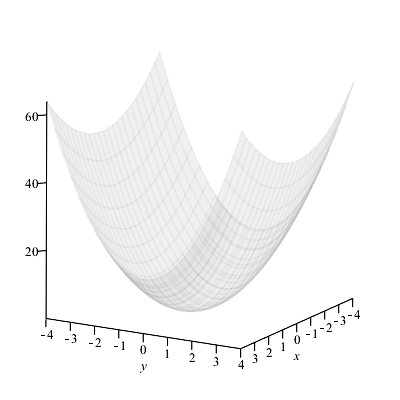
\includegraphics{10_6_Grad_ex_surface}}
  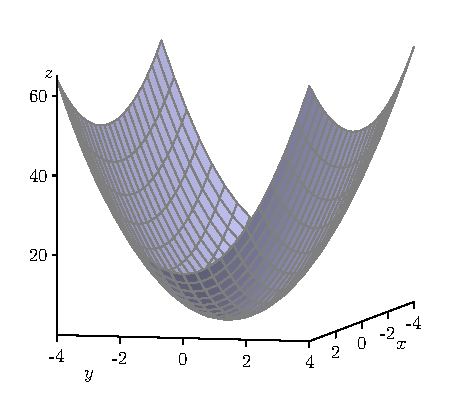
\includegraphics{figures/fig_10_6_exercise_graph.eps}
\end{center}
\caption{The surface for $f(x,y) = x^2+3y^2$.}
\label{F:10.6.Grad_ex}
\end{minipage} \hspace{0.5in}
\begin{minipage}{2.5in}
\begin{center}
%\resizebox{!}{2.2in}{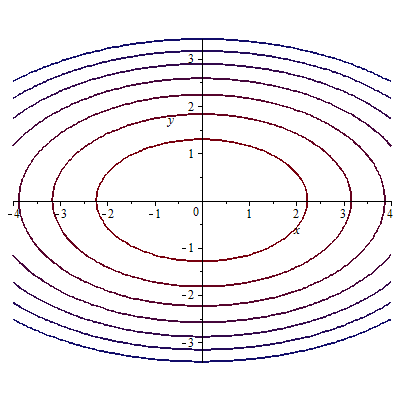
\includegraphics{10_6_Grad_ex_contours}}
  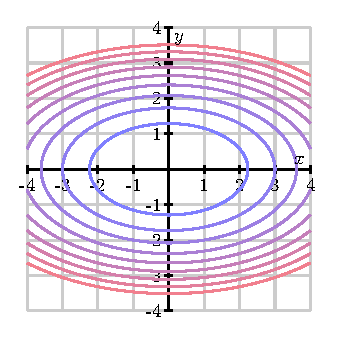
\includegraphics{figures/fig_10_6_exercise_contour.eps}
\end{center}
\caption{Contours for $f(x,y) = x^2+3y^2$.}
\label{F:10.6.Grad_ex_contours}
\end{minipage}
\end{center}
\end{figure}

	\item Find a direction $\vw$ for which the slope of the tangent line to the surface generated by $f$ at the point $(1,2)$ is zero in the direction $\vw$.

    \ea

\begin{exerciseSolution}
\ba 
   \item In this case we have
\[\nabla f = \langle f_x, f_y \rangle = \langle 2x, 6y \rangle.\]
 Evaluating $\nabla f$ at $(1,2)$ gives us
\[\nabla f(1,2) = \langle 2, 12 \rangle.\]

	\item The gradient shows the direction of greatest increase of $f$ at a point. An illustration of this direction at the point $(1,2,f(1,2))$ is shown in the figure below, with the gradient vector scaled appropriately to make it easier to plot. 
\begin{center}
\resizebox{!}{2.2in}{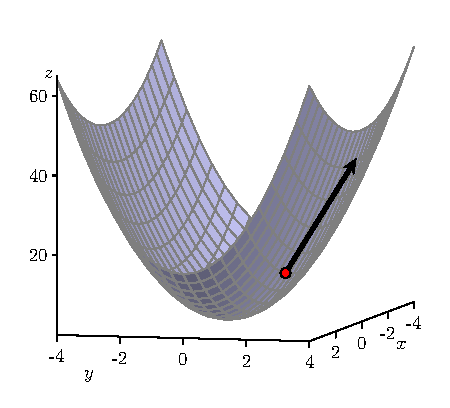
\includegraphics{figures/fig_10_6_Ex_surface_gradient}}
\end{center}

	\item The gradient shows the direction of greatest increase of $f$ at a point. The gradient is perpendicular to the level curves, and a picture of the unit vector in the direction of the gradient at $(1,2)$ is shown in the figure below, with the gradient vector scaled appropriately to make it easier to plot.  
\begin{center}
\resizebox{!}{2.2in}{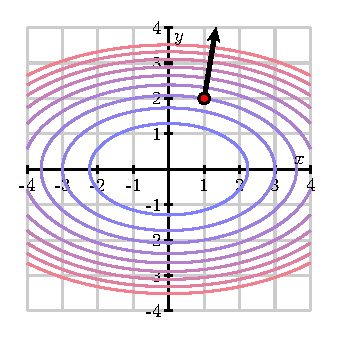
\includegraphics{figures/fig_10_6_Ex_contour_gradient}}
\end{center}

	\item We need to find a direction $\vw = \langle w_1, w_2 \rangle$ so that $D_{\vw} f(1,2) = \nabla f(1,2) \cdot \vw = 0$. Since $\nabla f (1,2)= \langle 2, 6 \rangle$, we need $w_1$ and $w_2$ to satisfy $2w_1+6w_2=0$. So $w_1=-3w_2$ and a direction for which the slope of the tangent line to the surface generated by $f$ at the point $(1,2)$ is zero in the direction $\vw$ is $\langle -3,1 \rangle$. 

\ea

\end{exerciseSolution}


\item The properties of the gradient that we have observed for functions of two variables also hold for functions of more variables.  In this problem, we consider a situation where there are three independent variables.  Suppose that the temperature in a region of space is described by
  $$
  T(x,y,z) = 100e^{-x^2-y^2-z^2}
  $$
  and that you are standing at the point $(1,2,-1)$.
  \ba
\item Find the instantaneous rate of change of the temperature in the direction of
  $\vv=\langle 0, 1, 2\rangle$ at the point $(1,2,-1)$.  Remember that you should first find a
  {\em unit} vector in the direction of $\vv$.

\item In what direction from the point $(1,2,-1)$ would you move to cause the temperature to
  decrease as quickly as possible?

\item How fast does the temperature decrease in this direction?

\item Find a direction in which the temperature does
  not change at $(1,2,-1)$.

  \ea


\begin{exerciseSolution}
  \ba
\item A unit vector in the direction of $\vv$ is $\vu = \frac{1}{\sqrt{5}} \vv$. The instantaneous rate of change of the temperature in the direction of
  $\vv=\langle 0, 1, 2\rangle$ is then
\begin{align*}
\left| \nabla T(1,2,-1) \cdot \vu \right| &= \left| \langle T_x(1,2,-1), T_y(1,2,-1), T_z(1,2,-1) \rangle \cdot \vu \right| \\
	&= \left| \left\langle -200e^{-6}, -400e^{-6}, 200e^{-6} \right\rangle \cdot \frac{1}{\sqrt{5}} \langle 0,1,2\rangle \right| \\
	&= \left|-80\sqrt{5}\left\langle 0, e^{-6}, -e^{-6} \right\rangle \right| \\
	&= 80\sqrt{5}\sqrt{2}e^{-6} \\
	&\approx 0.627. \\
\end{align*}

\item To cause the temperature to decrease as quickly as possible we move in the direction of 
\[-\nabla T(1,2,-1) = \left\langle 200e^{-6}, 400e^{-6}, -200e^{-6} \right\rangle \approx \langle 0.5, 1, -0.5 \rangle.\]


\item The rate of change of the temperature in this direction is 
\[\left|\nabla T(1,2,-1) \right| =  200 \sqrt{6}e^{-6} \approx 1.21.\]
So the temperature decreases at approximately 1.21 in this direction.

\item Let $\vu = \langle u_1, u_2, u_3 \rangle$ be a vector in a direction in which the temperature does not change. Then
\begin{align*}
0 &= \nabla T(1,2,-1) \cdot \vu \\
	&= \left\langle -200e^{-6}, -400e^{-6}, 200e^{-6} \right\rangle \cdot \langle u_1, u_2, u_3 \rangle \\
	&= -200e^{-6}(u_1+2u_2-u_3).
\end{align*}
So a direction in which the temperature does not change is the direction of the vector $\langle -1,1,1 \rangle$. 


  \ea
\end{exerciseSolution}

\item Figure \ref{F:10.6.gradient.field} shows a plot of the gradient
  $\nabla f$ at several points for some function $f(x,y)$.

  \begin{figure}[ht]
    \begin{center}
     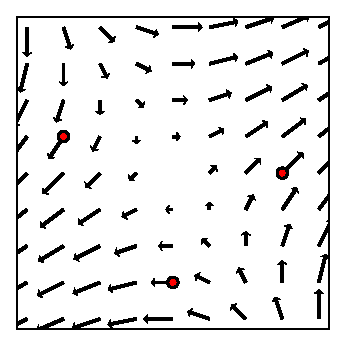
\includegraphics{figures/fig_10_6_gradient_field.eps}
    \end{center}	
    \caption{The gradient $\nabla f$.}
    \label{F:10.6.gradient.field}
  \end{figure}

  \ba
\item Consider each of the three indicated points, and draw, as best
  as you can, the contour through that point.

\item Beginning at each point, draw a curve on which $f$ is continually
  decreasing. 

  \ea

\begin{exerciseSolution}
  \ba
\item Since the gradient at a point is orthogonal to the contour at that point, the contours through the indicated points are drawn orthogonal to the gradients. This is illustrated in the figures below.

\begin{center}
\resizebox{!}{1.5in}{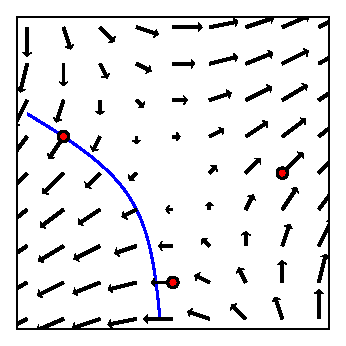
\includegraphics{figures/fig_10_6_Ex_4_a_1}} \hspace{0.1in} \resizebox{!}{1.5in}{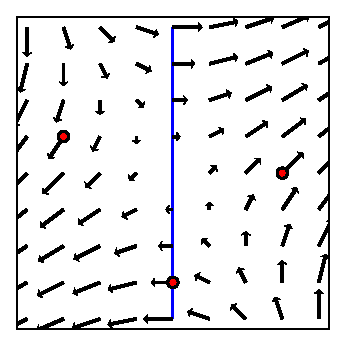
\includegraphics{figures/fig_10_6_Ex_4_b_1}}  \hspace{0.1in} \resizebox{!}{1.5in}{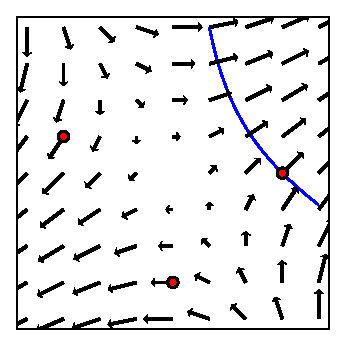
\includegraphics{figures/fig_10_6_Ex_4_c_1}}
\end{center}


\item The gradient points in the direction of the greatest increase of the function, so a curve that moves in the direction opposite the gradient is a curve on which $f$ is decreasing. This is illustrated in the figures below.

\begin{center}
\resizebox{!}{1.5in}{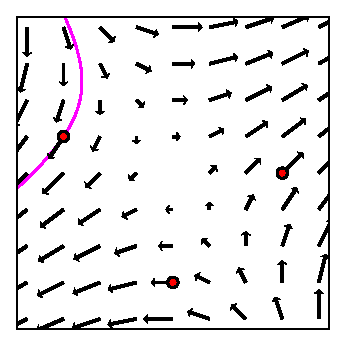
\includegraphics{figures/fig_10_6_Ex_4_a_2}} \hspace{0.1in} \resizebox{!}{1.5in}{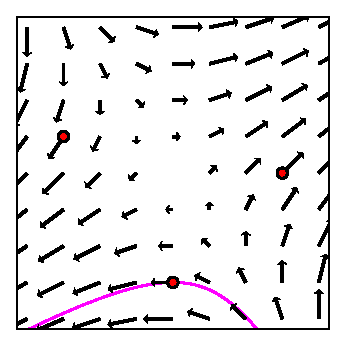
\includegraphics{figures/fig_10_6_Ex_4_b_2}}  \hspace{0.1in} \resizebox{!}{1.5in}{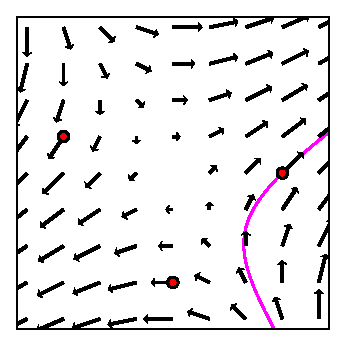
\includegraphics{figures/fig_10_6_Ex_4_c_2}}
\end{center}
  \ea
\end{exerciseSolution}

\end{exercises}

\afterexercises


\clearpage
